% This is samplepaper.tex, a sample chapter demonstrating the
% LLNCS macro package for Springer Computer Science proceedings;
% Version 2.21 of 2022/01/12
%
\documentclass{llncs}
%
\usepackage[T1]{fontenc}
% T1 fonts will be used to generate the final print and online PDFs,
% so please use T1 fonts in your manuscript whenever possible.
% Other font encondings may result in incorrect characters.
%
\usepackage{graphicx}
\usepackage{amsmath}
\usepackage{subcaption}
\usepackage{microtype}
% Used for displaying a sample figure. If possible, figure files should
% be included in EPS format.
%
% If you use the hyperref package, please uncomment the following two lines
% to display URLs in blue roman font according to Springer's eBook style:
%\usepackage{color}
%\renewcommand\UrlFont{\color{blue}\rmfamily}
%\urlstyle{rm}
%
\PassOptionsToPackage{hidelinks}{hyperref}
\usepackage{orcidlink}

\usepackage[style=apa, backend=biber, sortcites=false]{biblatex}

\setlength{\parskip}{0pt plus 0pt minus 0pt}

% Add the bib resource
\addbibresource{thebiblio.bib}

% Quitar sangría en bibliografía
\setlength{\bibhang}{0pt}
\setlength{\bibitemsep}{6pt}

% URLs en negro
\usepackage{xcolor}
\hypersetup{urlcolor=black}

\begin{document}
%
% ENGLISH VERSION
\title{\emph{Speckle} Noise Removal in SAR Images using Autoencoders}

%\titlerunning{Abbreviated paper title}
% If the paper title is too long for the running head, you can set
% an abbreviated paper title here
%
% For anonymous review, the author section has been commented out.
%\author{Bianca Balzarini\inst{1}\orcidlink{0000-0002-7483-2868} \and
%Juliana Gambini\inst{2,3,1}\orcidlink{0000-0002-4534-1402}}
%
%\authorrunning{B. Balzarini et al.}
% First names are abbreviated in the running head.
% If there are more than two authors, 'et al.' is used.
%
%\institute{Instituto Tecnológico de Buenos Aires, Bueno Aires, Argentina
%\email{bbalzarini@itba.edu.ar}\\
% \and
%LIDEC, Universidad Nacional de Hurlingham, Pcia. de Buenos Aires, Argentina\\
%\email{juliana.gambini@unahur.edu.ar} \\
%\and
%CPSI, Universidad Tecnológica Nacional, Regional Buenos Aires}

% Add empty author and institute to avoid compilation errors
\author{}
\institute{}
%
\maketitle              % typeset the header of the contribution
%
\begin{abstract}
Synthetic Aperture Radar (SAR) images are fundamental for Earth observation due to their ability to acquire data
independently of weather and lighting conditions. However, these images are affected by speckle noise, a
multiplicative granular pattern that degrades their quality and makes them difficult to automatically interpret.
This work presents an approach for speckle removal using convolutional autoencoders. The main innovation lies in
the use of the $\mathcal{G}_I^0$ distribution  to synthetically generate pairs of noisy and clean images for
supervised training, adequately modeling the statistical characteristics of real speckle noise.
In addition, we developed a flexible file-based configuration system that facilitates experimentation with
different network architectures.
Experimental outcomes reveal that deeper network architectures achieve better results with no evidence of
overfitting.
Models trained on synthetic data showed good performance on synthetic test images, but limitations in generalizing
to actual SAR images. To address this problem, we explored training with pairs of real images obtained through time
averaging, achieving significant improvements and performance comparable to other known models.

% keywords in lowercase
\keywords{aperture synthetic radar, speckle noise, autoencoders.}
\end{abstract}

% SPANISH VERSION
% Clear the previous title info and set Spanish version

% Spanish title and abstract
\begin{center}
\vspace{1cm}
{\Large \bfseries\boldmath Eliminación de Ruido \emph{Speckle} en Imágenes SAR utilizando Autoencoders}

\vspace{0.5cm}
\end{center}

\begin{abstract}
Las imágenes de Radar de Apertura Sintética (SAR: Synthetic Aperture Radar) son fundamentales para la observación
de la Tierra debido a su capacidad de adquisición independiente de las condiciones
climáticas y de iluminación. Sin embargo, estas imágenes se ven afectadas por el ruido \emph{speckle},
un patrón granular multiplicativo que degrada su calidad, y dificulta su interpretación.
Este trabajo presenta un enfoque para la eliminación de ruido \emph{speckle} mediante
el uso de autoencoders convolucionales. La principal innovación radica en el uso de la distribución
$\mathcal{G}_I^0$ para generar sintéticamente pares de imágenes ruidosas y limpias destinadas
al entrenamiento supervisado, modelando adecuadamente las características estadísticas del ruido
\emph{speckle} real. Complementariamente, desarrollamos un sistema flexible basado en archivos
de configuración que facilita la experimentación con diferentes arquitecturas de redes.
Los experimentos revelan que las arquitecturas más profundas obtienen consistentemente
mejores resultados sin evidencia de overfitting.

 Los modelos entrenados con datos sintéticos
mostraron buen desempeño en imágenes de prueba sintéticas, pero limitaciones en la generalización a imágenes SAR reales. Para abordar este problema, exploramos el entrenamiento con pares de
imágenes reales obtenidas mediante promediado temporal, logrando mejoras significativas
y desempeño comparable a otros ya conocidos.
%Este trabajo establece las bases para el uso de autoencoders en el filtrado de ruido \emph{speckle} y
%demuestra tanto el potencial como las limitaciones de los datos sintéticos generados mediante
%modelos estadísticos.


% palabras clave en minúsculas
\keywords{radar de apertura sintética (SAR), ruido speckle, autoencoders.}
\end{abstract}


\vspace{0.5cm}
\setcounter{page}{1}

\section{Introduction}
\label{sec:introduction}

Synthetic Aperture Radar (SAR) is a highly effective remote sensing technology capable of generating high-resolution
images of the Earth's surface regardless of weather or lighting conditions. This makes SAR imagery an invaluable
tool for applications ranging from environmental monitoring to terrain change detection and disaster management.
However, a significant drawback of SAR images is the inherent presence of speckle noise. Unlike the additive noise
common in optical imagery, speckle is a multiplicative, non-Gaussian phenomenon resulting from the coherent
interference of radar waves scattered by surface elements. This granular noise severely degrades the visual quality
of SAR images and complicates subsequent analysis and interpretation tasks.

Classical speckle mitigation techniques include adaptive filters (Lee, Frost) \parencite{lee1980digital, frost1982model}, wavelets \parencite{zhang2017nonmodel}, and non-local methods like SAR-BM3D \parencite{parrilli2012nonlocal}. These struggle to balance noise reduction with detail preservation. Deep learning, particularly CNNs and Autoencoders, has revolutionized image denoising \parencite{zhang2018dilated,lattari2019deep,vitale2021multiobjective,cardona2025optimization} using supervised learning with large datasets of paired noisy-clean images. Since perfectly noise-free SAR images are hard to aquire, synthetic data generation is essential, either by injecting simulated noise or averaging temporal images \parencite{vasquez2024labeled}, though the latter is scarce.

The efficacy of supervised deep learning depends heavily on simulated noise realism. Existing literature often uses simple statistical models (Gamma, Rayleigh), which are computationally convenient but limited. The Rayleigh distribution, for instance, is accurate only for homogeneous areas like pasturelands \parencite{lattari2019deep}, failing to capture complex statistical properties in heterogeneous terrain (urban, vegetation). This lmits generalization capability of the trained networks.

To address this gap, this paper proposes the use of $\mathcal{G}_I^0$ distribution for speckle simulation. The $\mathcal{G}_I^0$ distribution is renowned for accurately modeling speckle across diverse surface roughness and heterogeneous clutter \parencite{originalGI0}. Despite proven accuracy in SAR statistical modeling, its integration into synthetic deep-learning training pipelines remains underexplored. This work investigates how $\mathcal{G}_I^0$-based data preparation enhances autoencoder robustness and generalization, validated on both synthetic and actual SAR images using standard metrics.

Our main contributions are: (i) integrating the $\mathcal{G}_I^0$ model into a synthetic data pipeline for autoencoder training; (ii) a systematic evaluation of 25 autoencoder configurations driven by flexible config files; and (iii) empirical evidence that fine-tuning on actual SAR pairs substantially improves generalization.

This paper is organized as follows: Section 2 describes the methodology (data generation and architecture); Section 3 presents experiments and comparisons; Section 4 provides the conclusions and outlines future work.

\section{Materials and Methods}\n\subsection{SAR Images}\n\subsection{Methods}

\section{Results}

The extensive experimentation, summarized in Table \ref{tab:autoencoder_configs}, allowed for a deep analysis of the different architectural configurations. In this section, we present the quantitative, qualitative, and comparative results of the most relevant models.

\subsection{Performance on Synthetic Data}

The models were initially evaluated based on their Mean Squared Error (MSE) on a synthetic test set of 1000 images, kept separate from the training data. Table \ref{tab:mse_results} summarizes the performance of the top-performing architectures and other relevant cases.

The results clearly indicate that deeper architectures with three convolutional layers (A13, A15, A16) achieved the best performance, with MSE values around $0.0023$. This suggests that a hierarchical feature extraction is crucial for effectively modeling and removing speckle noise. Notably, the dimensionality of the latent space in these top models ($128$ or $256$) also played a significant role.

Furthermore, we observed that training duration did not linearly correlate with better performance. For instance, model A16, trained for only 70 epochs, achieved a performance nearly identical to A15 (trained for 500 epochs), suggesting that well-designed architectures can converge rapidly. This is a key finding, as it points towards more efficient training strategies. Several models, particularly shallower ones with long training times (e.g., A4), exhibited signs of overfitting, with a test MSE more than 25\% higher than their final training MSE.

\begin{table}[htbp]
\centering
\caption{Test MSE results for a selection of autoencoder configurations, ordered by performance. The table highlights the best models, an underperforming one, and a case with significant overfitting.}
\label{tab:mse_results}
\scriptsize
\begin{tabular}{|c|c|c|c|c|}
\hline
\textbf{Rank} & \textbf{Config.} & \textbf{Architecture Details} & \textbf{Test MSE} & \textbf{Comment} \\
\hline
1 & A15 & 3 Conv, 256 Dim, 500 Epochs & 0.002319 & Best performance \\
2 & A13 & 3 Conv, 128 Dim, 500 Epochs & 0.002346 & Excellent performance \\
3 & A16 & 3 Conv, 256 Dim, 70 Epochs  & 0.002348 & Best short-training model \\
4 & A7  & 2 Conv, 128 Dim, 500 Epochs & 0.002433 & Best 2-layer model \\
... & ... & ... & ... & ... \\
16 & A4 & 1 Conv, 32 Dim, 500 Epochs  & 0.002781 & High overfitting (+28.5\%) \\
... & ... & ... & ... & ... \\
23 & A1 & 1 Conv+Pool, 32 Dim, 5 Epochs & 0.005695 & Underperforming base model \\
\hline
\end{tabular}
\end{table}

\subsection{Visual Assessment and Architectural Insights}

Quantitative metrics are essential, but a visual assessment is crucial to understand the filter's behavior. Figure \ref{fig:imtest_A15} shows the result of applying the best-performing model, A15, to a sample synthetic test image.

The autoencoder demonstrates a remarkable ability to reduce speckle and reconstruct the mean gray levels of the homogeneous areas. However, the filtered image is not a perfect replica of the clean target. The model tends to introduce smooth, spatially correlated patterns, a common artifact of convolutional networks that are trained to find structure in images. This shows a fundamental challenge: the network struggles to distinguish between the speckle noise to be removed and the random texture inherent to the backscatter signal, which should be preserved. This behavior was consistent across all high-performing architectures.

\begin{figure}[htbp]
    \centering
    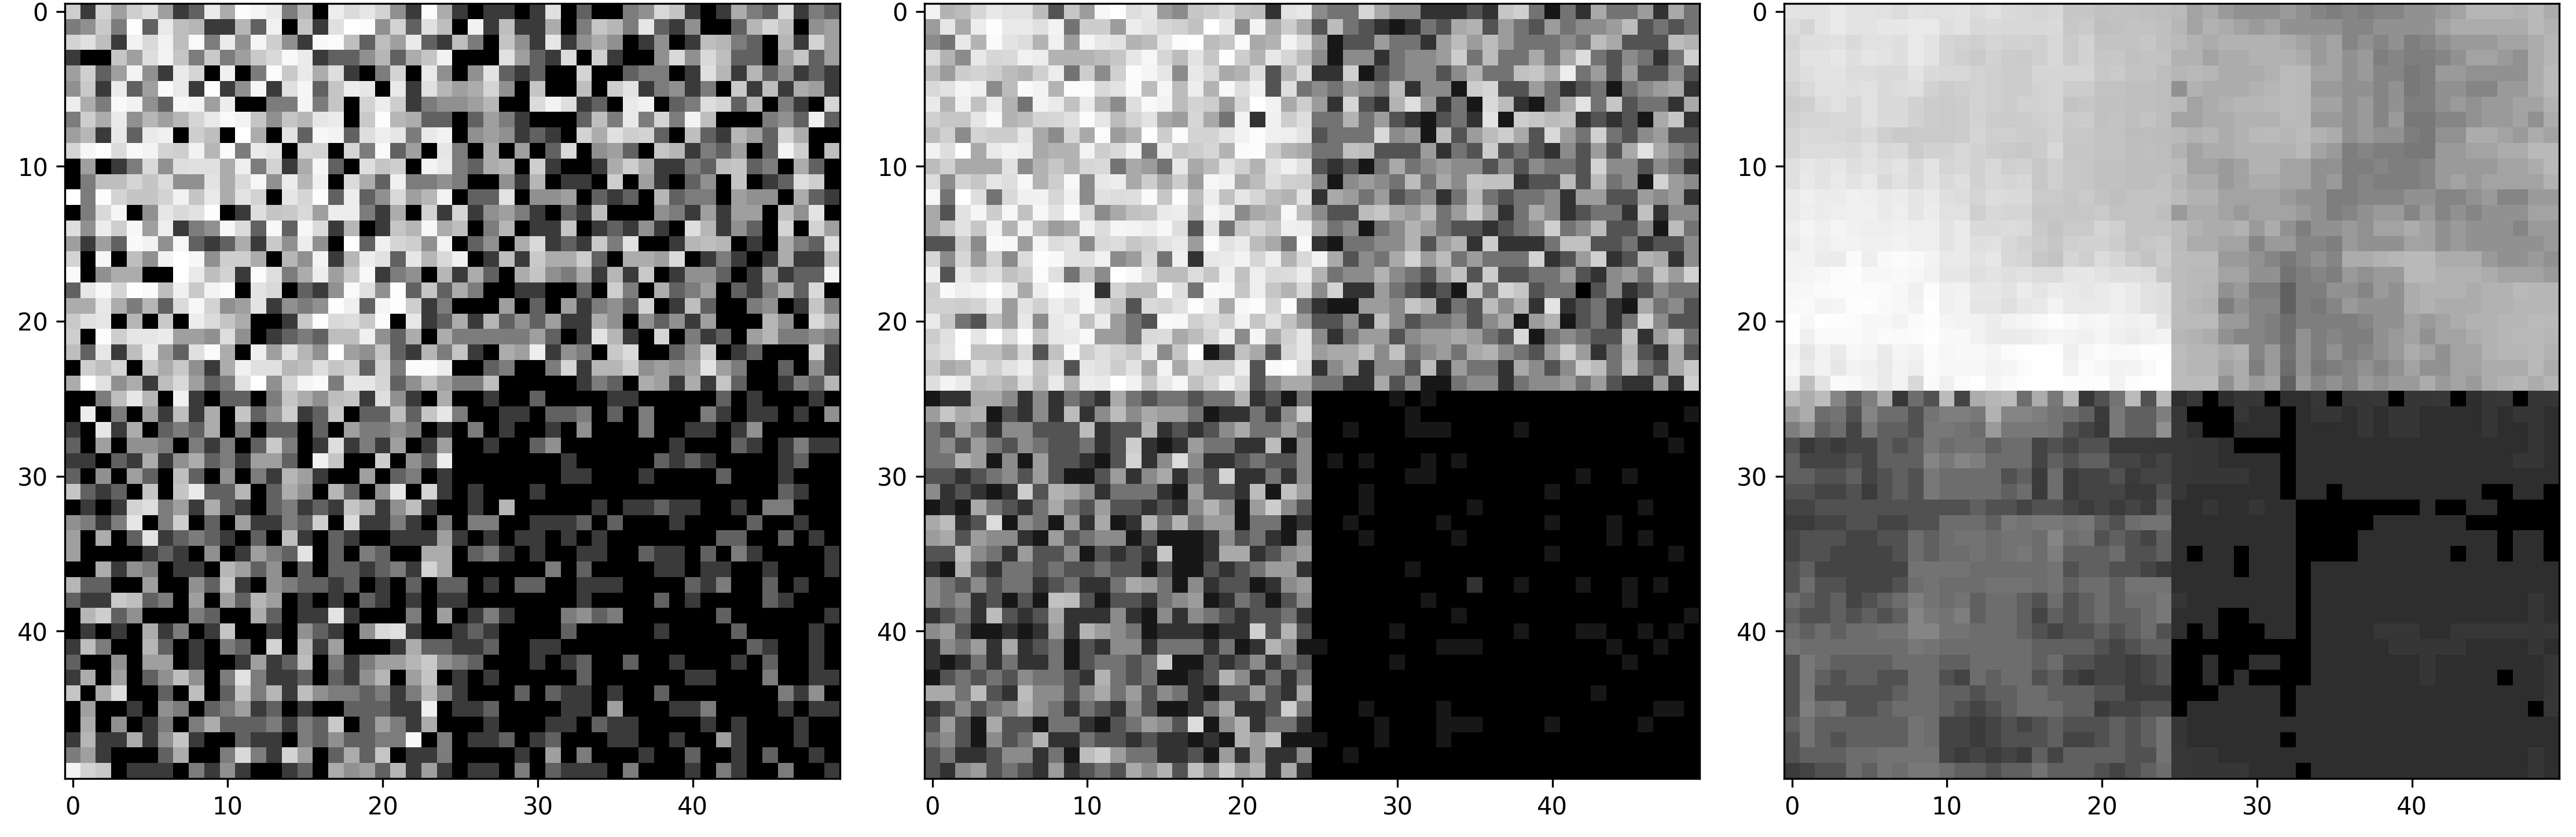
\includegraphics[width=0.9\textwidth]{Images/imtest_A15.png}
    \caption{Visual result of the A15 filter on a synthetic test image. From left to right: filtered output, original clean target, and noisy input. The model effectively removes noise but introduces artificial smoothness.}
    \label{fig:imtest_A15}
\end{figure}

\subsection{Performance on Real SAR Images}
To assess the generalization capabilities of our approach, the best model (A15) was applied to real SAR images. Figure \ref{fig:sar_munich_filtered} shows the result on a complex urban scene of Munich.

The filter successfully reduces a significant amount of the visible speckle, especially in smoother regions like parks or large rooftops. However, the model's limitations become apparent. Having been trained exclusively on simple, artificially generated quadrant images, the autoencoder did not learn the complex textures and structures inherent to real-world SAR data. As a result, it tends to over-smooth fine details and can sometimes create artifacts that do not correspond to the underlying scene. This highlights a key trade-off: while synthetic data allows for controlled training and evaluation, it may not equip the model with the robustness needed for the variability of real-world scenarios.

\begin{figure}[htbp]
    \centering
    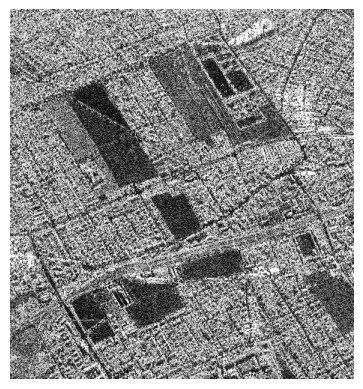
\includegraphics[width=0.7\textwidth]{Images/sar_munich.jpg}
    \caption{Application of the A15 filter to the original real SAR image of Munich (shown). On applying the filter, speckle is visibly reduced, particularly in homogeneous regions. However, as the model was trained on synthetic data, it tends to over-smooth complex textures and fine details present in the real scene.}
    \label{fig:sar_munich_filtered}
\end{figure}

\subsection{Statistical Evaluation and Comparative Analysis}

Finally, we performed a comparative analysis using the statistical figure of merit $\mathcal{M}$ described in the methods section, which combines mean preservation and residual structure analysis. We compared our best-performing autoencoders against the well-established Lee filter, a standard benchmark in speckle reduction. The results are summarized in Table \ref{tab:stat_results}.

\begin{table}[htbp]
\centering
\caption{Statistical figure of merit $\mathcal{M}$ for the top autoencoders compared to the Lee filter. A lower value indicates better overall performance.}
\label{tab:stat_results}
\begin{tabular}{|l|c|}
\hline
\textbf{Filter} & \textbf{Figure of Merit ($\mathcal{M}$)} \\
\hline
\textbf{Autoencoder A15} & \textbf{0.69} \\
Autoencoder A16 & 0.72 \\
Lee Filter (7x7) & 0.85 \\
\hline
\end{tabular}
\end{table}

The results show that our proposed autoencoder architectures, particularly A15, outperform the traditional Lee filter. They achieve a better balance of noise reduction (contributing to a higher ENL) and structure preservation, as captured by the lower $\mathcal{M}$ value. This demonstrates that, despite the limitations observed, the data-driven approach of a convolutional autoencoder can provide a superior despeckling performance compared to classic filtering techniques.

\section{Conclusions and Future Work}
\label{chap:conclusions}

In this work, we explored the use of autoencoders for speckle noise reduction in SAR images, presenting original contributions in both the training data generation methodology and the development of flexible tools for experimenting with different architectures. We demonstrated that it is possible to use the $\mathcal{G}_I^0$ distribution to generate synthetic training data for training autoencoders capable of filtering speckle noise, although with limitations in their generalization to actual images. Our experiments consistently reveal that deeper and more complex architectures yield better results. And we also achieved results similar to those of traditional filters. However, the superior performance observed with models trained directly on actual data underscores the importance of having training data that is representative of the application domain.

Our findings highlight a key dichotomy in the use of synthetic data: the $\mathcal{G}_I^0$ model offers a controllable environment for architecture development, but a gap remains with real SAR images. Thus, the strongest use of synthetic data is as a pre-training step to provide a statistical prior, followed by fine-tuning on a smaller real SAR dataset. This two-stage strategy can combine synthetic fidelity with real data adaptation and should be validated using both reconstruction error and speckle-preserving metrics.

Future research will focus on exploring more sophisticated architectures, such as U-Net and attention-based models, and on formalizing the hybrid training strategy suggested by our results. A promising next step is to evaluate transfer learning by pre-training on large synthetic $\mathcal{G}_I^0$ datasets and then fine-tuning on smaller real SAR sets. This may involve layered fine-tuning, mixed-domain batches, and hybrid losses that balance reconstruction accuracy with statistical consistency. We also plan to refine synthetic generation with greater spatial diversity and richer texture variations. In addition, although this work compares the proposed autoencoder approach with the classical Lee filter, a more complete evaluation should include modern speckle reduction algorithms such as the FANS filter. A rigorous comparison with other state-of-the-art methods remains a priority for future work. Finally, we will extend the proposed methodology to more complex data, including polarimetric and multi-temporal SAR images, to assess its performance in a broader range of applications. While the use of Mean Squared Error (MSE) as the loss function provided a solid baseline for this study, we acknowledge its limitations in capturing the perceptual and textural nuances of SAR imagery. As noted, optimizing for MSE can lead to a 'regression to the mean,' resulting in blurred reconstructions that may lack high-frequency details. Our decision was pragmatic, aimed at first validating our data generation and architectural hypotheses in a controlled manner. Thus, our work separates the optimization objective (MSE) from the evaluation criteria: MSE is used to train stable reconstructions, while the speckle-specific metrics verify that the output maintains the desired statistical behavior.

For future work, we plan to explore more advanced loss functions. A promising direction is the development of a custom perceptual loss tailored for SAR images, which would require pre-training a feature extractor on a large SAR dataset. This type of loss compares learned features rather than individual pixels, helping to preserve textural and structural details that MSE alone tends to smooth.

Another direction is to incorporate terms that measure the match between distributions, such as those used in Generative Adversarial Networks (GANs) or Wasserstein-based losses. Implementing this would require a discriminative component or GAN-style architecture capable of learning the statistical distribution of real clean SAR images, which is more complex than our current MSE-based framework.

The positive results from our current MSE-based models provide a strong foundation for these future explorations, which we believe will yield significant improvements in reconstruction quality.
In conclusion, this work establishes a solid foundation for using autoencoders for speckle noise reduction in SAR images, demonstrating the potential of combining statistical models with deep learning to address classic radar image processing problems.

\begin{sloppypar}
\printbibliography
\end{sloppypar}

\end{document}
